\documentclass[12pt,a4paper]{article}

\usepackage[margin=1.8cm]{geometry}
\usepackage{graphicx}
\usepackage{float}
\usepackage{titlesec}
\usepackage{amsmath}
\usepackage{enumitem}
\usepackage{booktabs}
\usepackage{caption}

% ---------- Compact Layout ----------
\linespread{0.97}            % line height thấp vừa phải
\setlength{\parskip}{4pt}    % khoảng cách giữa các đoạn
\setlength{\parindent}{0pt}  % bỏ thụt đầu dòng
\setlist[itemize]{noitemsep, topsep=2pt}

% ---------- Section Spacing ----------
\titlespacing*{\section}{0pt}{10pt}{6pt}
\titlespacing*{\subsection}{0pt}{8pt}{4pt}

\titleformat{\section}{\large\bfseries}{\thesection}{1em}{}
\titleformat{\subsection}{\normalsize\bfseries}{\thesubsection}{1em}{}

\begin{document}

% -------------------- COVER PAGE --------------------

\begin{center}
    \textbf{\Large Subject: DAM501.22}

    \vspace{0.5cm}

    \textbf{\Large Data Mining Project Report}

    \vspace{0.5cm}

    \textbf{\Huge Customer Segmentation (Clustering)}

    \vspace{0.8cm}

    \textbf{Nguyen Nhut Minh} \\
    Student ID: 25MS23283 \\
    Supervisor: Tran Minh Trung \\[1cm]

    \textit{March 03, 2026}
\end{center}

\vspace{0.8cm}
\hrule
\vspace{0.8cm}

% -------------------- CONTENT --------------------

\section{Identify the Business Problem}

\subsection{Business Context}

In a competitive retail environment, shopping malls must understand customer behavior in order to design effective marketing strategies. Customers differ significantly in terms of age, income level, and purchasing behavior. Without a clear segmentation strategy, marketing campaigns may be inefficient, resulting in wasted budget and missed opportunities.

The management of the mall aims to better understand their customer base and group customers into meaningful segments. These segments can then be used to personalize promotions, loyalty programs, and targeted advertisements.

\subsection{Business Objective}

The main objective of this project is:

\begin{itemize}
    \item To segment customers into homogeneous groups based on their demographic and behavioral characteristics in order to support marketing decision-making.
\end{itemize}

Specifically, the mall management would like to:

\begin{itemize}
    \item Identify high-value customers.
    \item Detect customers with high spending behavior relative to income.
    \item Discover potential customer groups for targeted promotions.
    \item Improve marketing efficiency through data-driven segmentation.
\end{itemize}

\subsection{Data Mining Perspective}

From a data mining perspective, this problem can be formulated as an unsupervised learning task because:

\begin{itemize}
    \item There is no predefined label indicating customer groups.
    \item The objective is to discover hidden structures within the data.
\end{itemize}

Therefore, clustering algorithms are appropriate for this task. The models considered in this project include:

\begin{itemize}
    \item K-Means Clustering
    \item Hierarchical Clustering (Agglomerative, Ward linkage)
\end{itemize}

Model performance will be evaluated using internal validation metrics such as the Silhouette Score and visual analysis (e.g., PCA projection and dendrogram).

\subsection{Expected Business Impact}

The output of this project will allow the organization to:

\begin{itemize}
    \item Design differentiated marketing strategies for each customer segment.
    \item Allocate promotional budgets more effectively.
    \item Improve customer retention and satisfaction.
    \item Increase overall profitability through targeted engagement.
\end{itemize}

% ----------------------------------------------------

\section{Prepare Data}

\subsection{Dataset Description}

The dataset used in this study is the \textit{Mall Customers} dataset, which is publicly available on Kaggle.\footnote{Mall Customers Dataset. Available at: \texttt{https://www.kaggle.com/datasets/vjchoudhary7/customer-segmentation-tutorial-in-python}} It contains demographic and behavioral information of 200 customers visiting a shopping mall.

The main attributes include:

\begin{itemize}
    \item \textbf{CustomerID}: Unique identifier for each customer.
    \item \textbf{Gender}: Male or Female.
    \item \textbf{Age}: Age of the customer.
    \item \textbf{Annual Income (k\$)}: Annual income measured in thousand dollars.
    \item \textbf{Spending Score (1--100)}: A score assigned by the mall based on customer purchasing behavior.
\end{itemize}

Since clustering focuses on behavioral patterns rather than identification, the \texttt{CustomerID} attribute is removed during preprocessing.

\subsection{Exploratory Data Analysis}

Before applying clustering algorithms, an exploratory data analysis (EDA) was performed to better understand the data distribution and relationships between variables.

Figure~\ref{fig:histograms} shows the distribution of the three numerical variables. The age distribution is right-skewed, indicating a larger proportion of younger customers. Annual income and spending score are approximately normally distributed.

\begin{figure}[H]
    \centering
    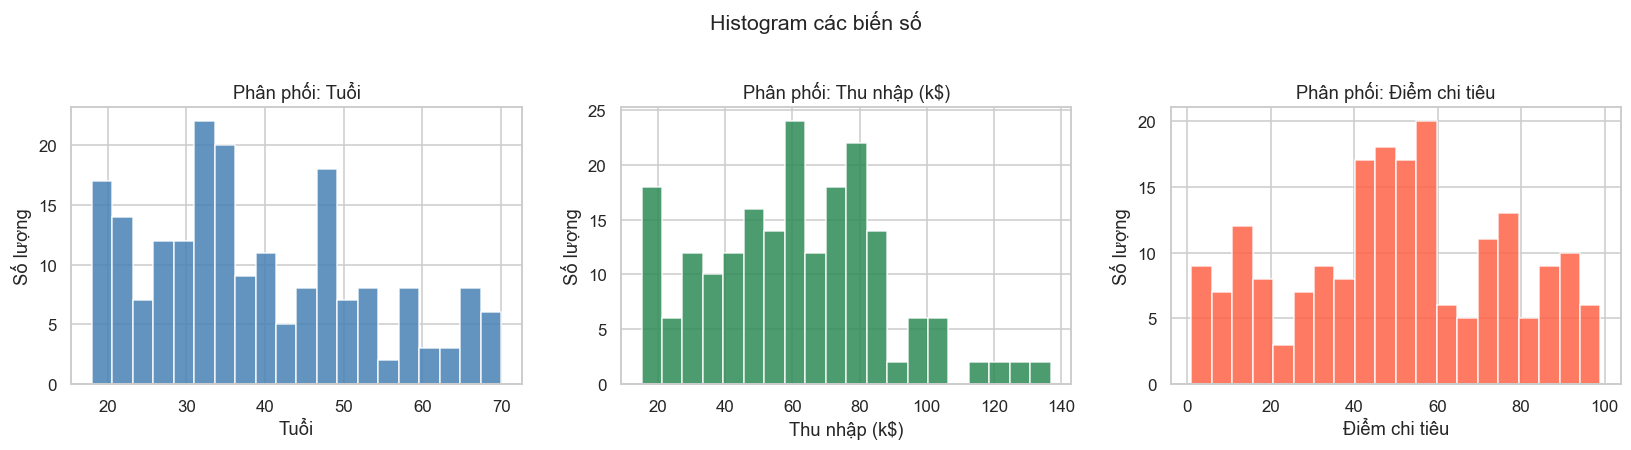
\includegraphics[width=\textwidth]{figures/fig_00.png}
    \caption{Distribution of Age, Annual Income, and Spending Score}
    \label{fig:histograms}
\end{figure}

Figure~\ref{fig:boxplot} presents the boxplots of each numerical feature grouped by gender. The distributions are similar across both genders, suggesting that gender alone does not strongly differentiate customer behavior.

\begin{figure}[H]
    \centering
    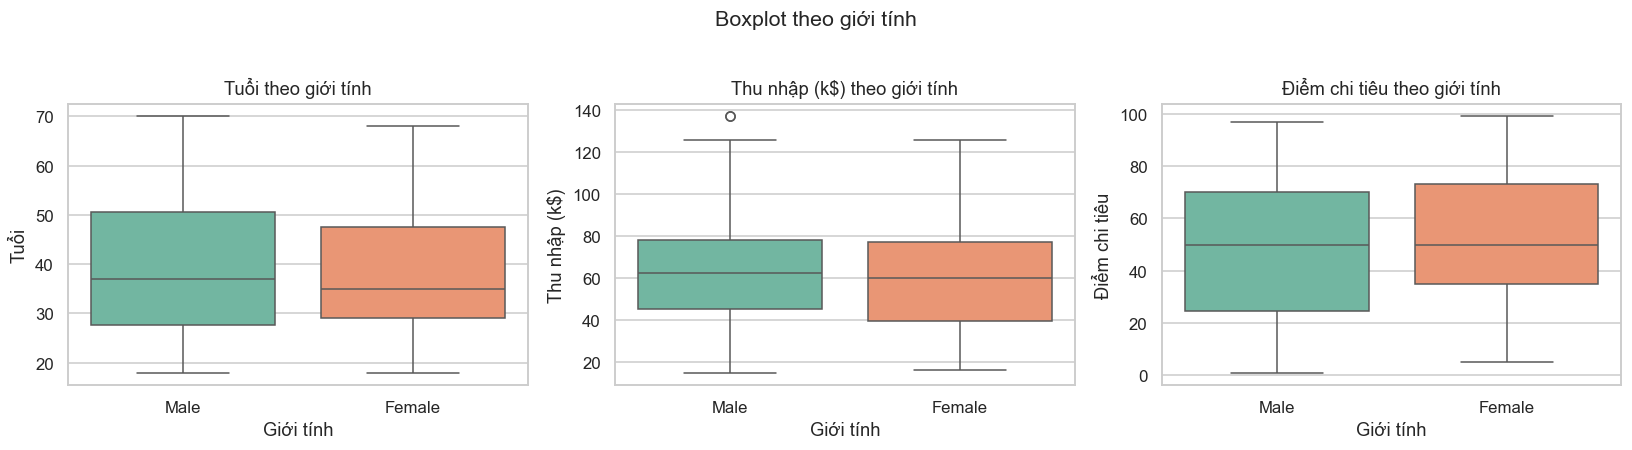
\includegraphics[width=\textwidth]{figures/fig_01.png}
    \caption{Boxplots of numerical features by gender}
    \label{fig:boxplot}
\end{figure}

Figure~\ref{fig:corr} shows the correlation heatmap and the scatter plot of Annual Income versus Spending Score. The scatter plot visually reveals the presence of approximately five natural groupings, which motivates the selection of $K = 5$ clusters.

\begin{figure}[H]
    \centering
    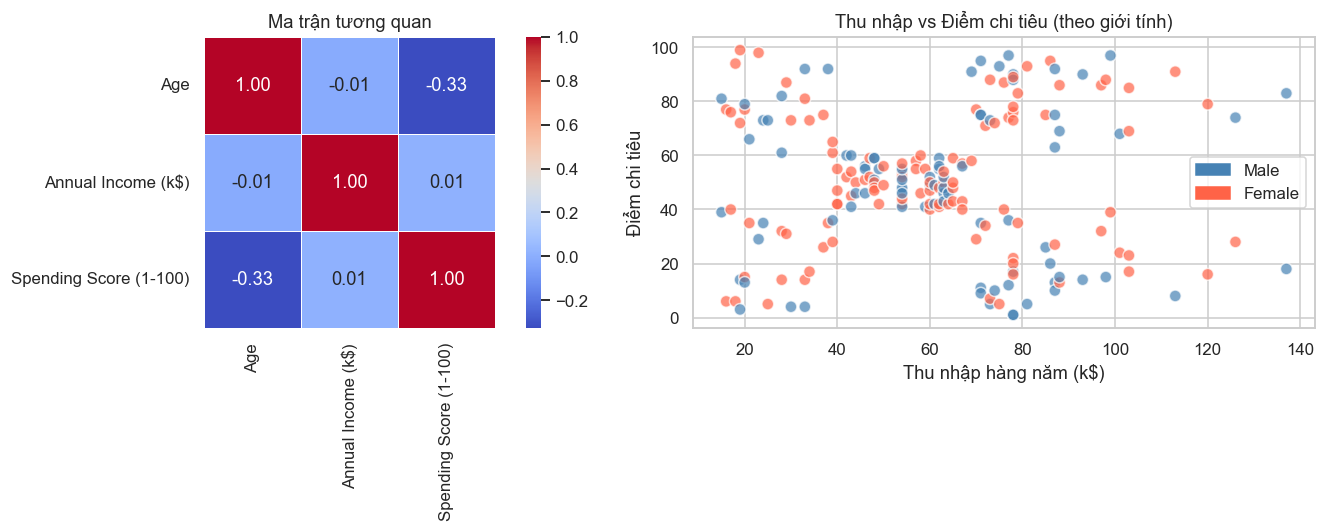
\includegraphics[width=\textwidth]{figures/fig_02.png}
    \caption{Correlation matrix and Income vs.\ Spending Score scatter plot}
    \label{fig:corr}
\end{figure}

\subsection{Data Cleaning}

The following preprocessing steps were performed:

\begin{itemize}
    \item Renaming columns for consistency and simplicity.
    \item Removing irrelevant attributes (e.g., CustomerID).
    \item Checking for missing values.
    \item Encoding categorical variables (e.g., Gender) into numerical format when necessary.
\end{itemize}

The dataset does not contain missing values, so no imputation was required.

\subsection{Feature Selection}

The selected features for clustering include:

\begin{itemize}
    \item Age
    \item Annual Income
    \item Spending Score
\end{itemize}

Optionally, the Gender attribute can be encoded and included in the clustering process to evaluate its influence on segmentation results.

\subsection{Feature Scaling}

Clustering algorithms are sensitive to differences in feature scales. For example:

\begin{itemize}
    \item Annual income may range from 15 to 140 (thousand dollars).
    \item Spending score ranges from 1 to 100.
    \item Age has a different numerical distribution.
\end{itemize}

If features are not normalized, attributes with larger numerical ranges may dominate the clustering process.

Therefore, \textbf{Standardization} was applied using the \texttt{StandardScaler}, transforming each feature as follows:

\[
z = \frac{x - \mu}{\sigma}
\]

where:
\begin{itemize}
    \item $x$ is the original feature value,
    \item $\mu$ is the mean,
    \item $\sigma$ is the standard deviation.
\end{itemize}

This transformation ensures that all features contribute equally to the clustering algorithm.

\subsection{Prepared Dataset}

After preprocessing and normalization, the final dataset is ready for:

\begin{itemize}
    \item Feature engineering,
    \item Clustering model training,
    \item Model evaluation and comparison.
\end{itemize}

% ----------------------------------------------------

\section{Create New Feature}

\subsection{Motivation}

While Annual Income and Spending Score provide useful information independently, they do not fully capture the relationship between earning capacity and purchasing behavior.

For example, two customers may have the same spending score, but one might have a significantly lower income. In such a case, the second customer could be considered relatively more engaged or more willing to spend compared to their financial capacity.

To better reflect this relationship, a new derived feature is introduced.

\subsection{Spending Score per Income}

A new feature named \textbf{Spending\_Score\_Per\_Income} is created to measure the relative spending behavior of a customer with respect to their income level.

The feature is defined as:

\[
\text{Spending\_Score\_Per\_Income} = \frac{\text{Spending Score}}{\text{Annual Income}}
\]

This transformation provides the following benefits:

\begin{itemize}
    \item Captures spending intensity relative to income.
    \item Highlights customers who spend aggressively despite lower income.
    \item Reduces bias toward customers with naturally higher income values.
\end{itemize}

This ratio-based feature normalizes spending behavior by income level, which helps the clustering algorithm detect customers who spend more aggressively relative to their financial capacity.

\subsection{Business Interpretation}

From a business perspective, this feature helps identify:

\begin{itemize}
    \item High-spending low-income customers (potentially highly engaged shoppers).
    \item Low-spending high-income customers (untapped premium segment).
    \item Balanced customers whose spending aligns with their income level.
\end{itemize}

This derived metric supports more nuanced segmentation compared to using raw attributes alone.

\subsection{Normalization of the New Feature}

Since this feature is ratio-based and may have a different numerical scale compared to other variables, it is also included in the standardization process.

After adding the new feature, the feature set used for clustering becomes:

\begin{itemize}
    \item Age
    \item Annual Income
    \item Spending Score
    \item Spending\_Score\_Per\_Income
\end{itemize}

All selected features are standardized to ensure equal contribution in the clustering process.

\subsection{Impact on Clustering}

By incorporating Spending\_Score\_Per\_Income, the clustering algorithm can better distinguish:

\begin{itemize}
    \item Customers with similar income but different spending behaviors.
    \item Customers with similar spending scores but different financial capacity.
\end{itemize}

This feature enhances the model's ability to uncover hidden behavioral patterns and improves the interpretability of the resulting customer segments.

% ----------------------------------------------------

\section{Train and Test Model}

\subsection{Clustering Approach}

Since the dataset does not contain predefined labels indicating customer groups, this problem is addressed using unsupervised learning techniques. Clustering algorithms are used to automatically identify patterns and group customers with similar characteristics.

In this project, two clustering algorithms are applied:

\begin{itemize}
    \item \textbf{K-Means Clustering}
    \item \textbf{Hierarchical Clustering (Agglomerative)}
\end{itemize}

These algorithms are widely used for customer segmentation because they can effectively discover natural groupings in data.

\subsection{Determining the Optimal Number of Clusters}

To determine the appropriate number of clusters, both the \textbf{Elbow Method} and the \textbf{Silhouette Score} are evaluated over $K \in \{2, \ldots, 10\}$.

The Elbow Method plots the Within-Cluster Sum of Squares (WCSS) against different values of $K$. The optimal $K$ corresponds to the ``elbow'' point where the rate of WCSS decrease slows significantly. The Silhouette Score measures cluster cohesion and separation, and is plotted to identify the $K$ that maximizes this metric.

Figure~\ref{fig:optk} shows both charts. The WCSS curve exhibits a clear elbow at $K = 5$, while the Silhouette chart also indicates $K = 5$ as a strong candidate in the context of domain interpretability. Based on these analyses, $K = 5$ is selected for both clustering models.

\begin{figure}[H]
    \centering
    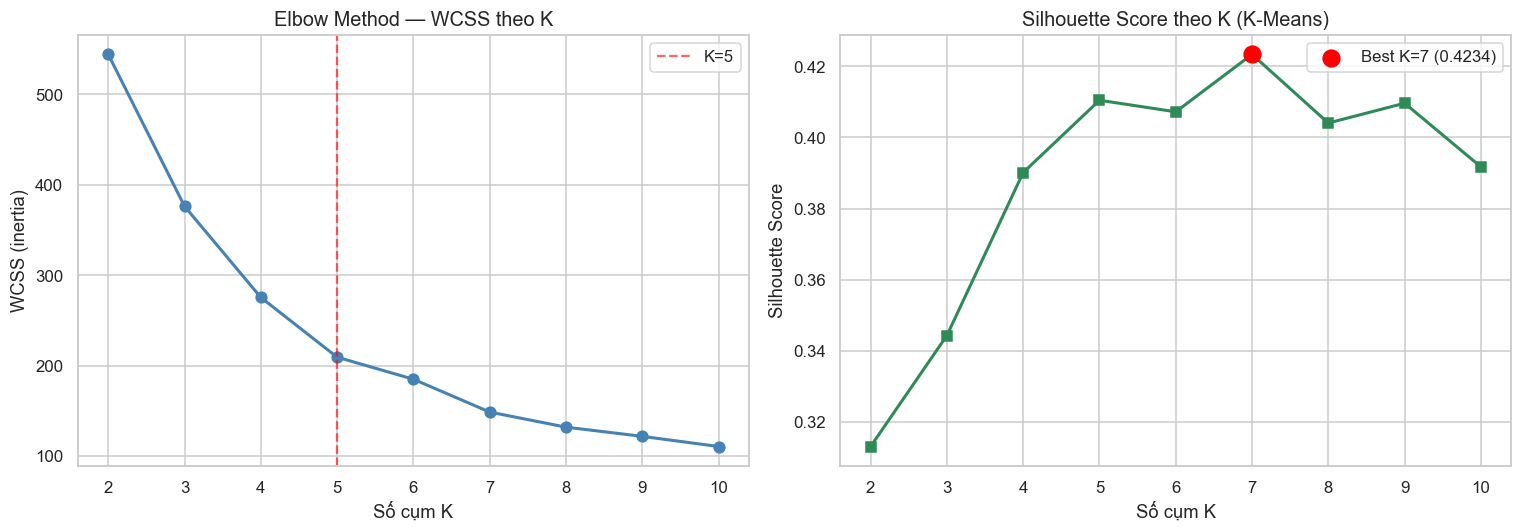
\includegraphics[width=\textwidth]{figures/fig_03.png}
    \caption{Elbow Method (WCSS) and Silhouette Score across $K = 2$ to $10$}
    \label{fig:optk}
\end{figure}

\subsection{K-Means Clustering}

K-Means is a centroid-based clustering algorithm that partitions the dataset into $K$ clusters. Each cluster is represented by a centroid, and each data point is assigned to the cluster with the nearest centroid.

The algorithm follows these main steps:

\begin{enumerate}
    \item Initialize $K$ cluster centroids randomly.
    \item Assign each data point to the nearest centroid.
    \item Recalculate centroids based on the mean of assigned points.
    \item Repeat the assignment and update steps until convergence.
\end{enumerate}

Figure~\ref{fig:kmeansscatter} shows the K-Means clustering result ($K = 5$) plotted on the two main feature axes. The centroids (marked with black ``$\times$'') are visible at the center of each cluster. The clusters are well-separated in the Income vs.\ Spending Score space, confirming the validity of the segmentation.

\begin{figure}[H]
    \centering
    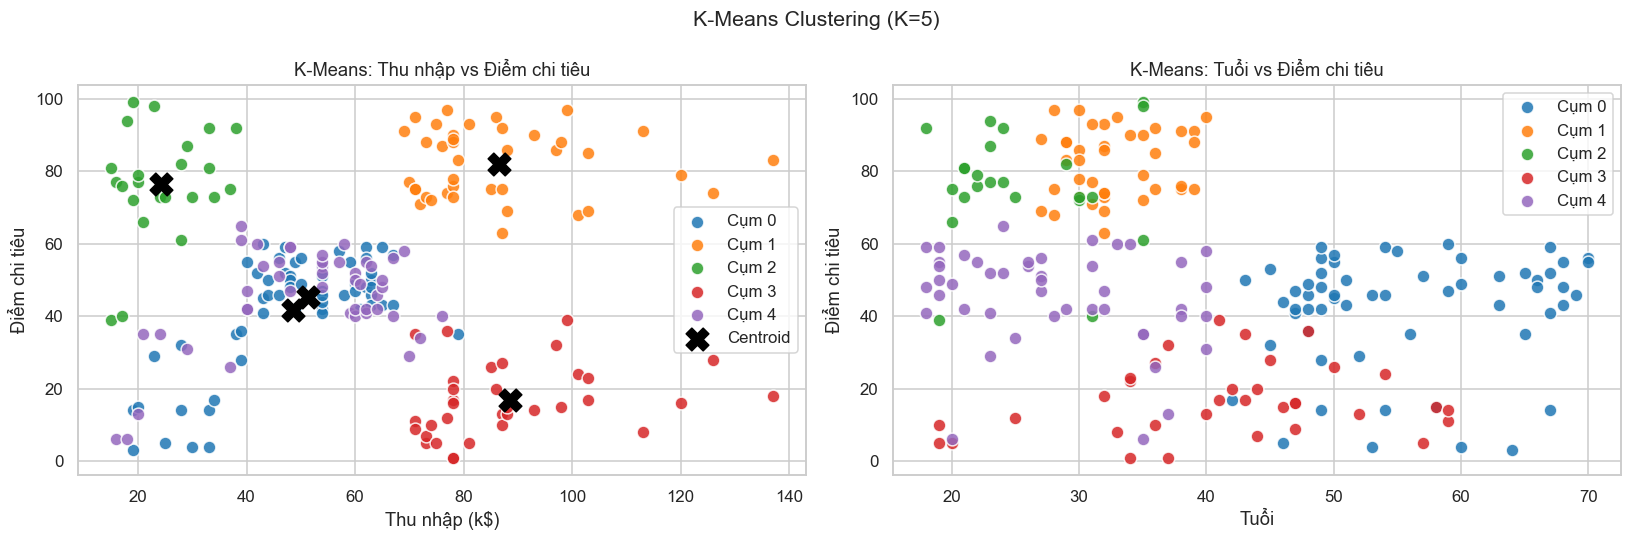
\includegraphics[width=\textwidth]{figures/fig_04.png}
    \caption{K-Means clustering result: Income vs.\ Spending Score (left) and Age vs.\ Spending Score (right)}
    \label{fig:kmeansscatter}
\end{figure}

Figure~\ref{fig:kmeanspca} presents the K-Means results projected onto a 2-dimensional PCA space. The first two principal components explain \textbf{78.4\%} of the total variance (PC1: 49.5\%, PC2: 28.9\%), confirming that the 2D projection is representative of the original feature space.

\begin{figure}[H]
    \centering
    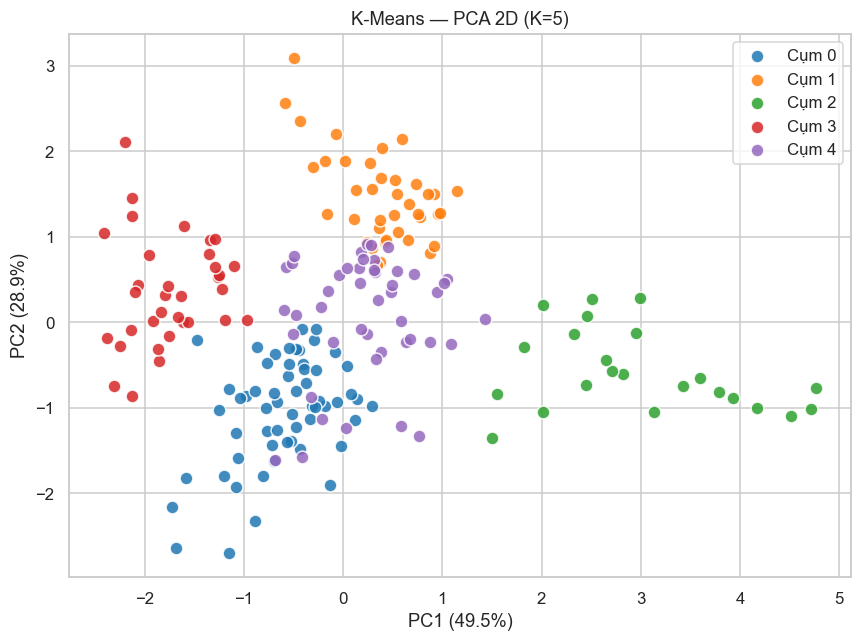
\includegraphics[width=0.65\textwidth]{figures/fig_05.png}
    \caption{K-Means result projected onto PCA 2D space (PC1 + PC2 = 78.4\% variance)}
    \label{fig:kmeanspca}
\end{figure}

The K-Means model performance metrics for $K = 5$ are:
\begin{itemize}
    \item Silhouette Score: \textbf{0.4105}
    \item Davies-Bouldin Index: \textbf{0.8508}
    \item WCSS (Inertia): \textbf{209.27}
    \item Cluster sizes: 58, 39, 23, 34, 46 customers
\end{itemize}

\subsection{Hierarchical Clustering}

Hierarchical clustering builds a hierarchy of clusters without requiring the number of clusters to be specified initially. In this project, the agglomerative approach is used.

Agglomerative clustering starts with each data point as its own cluster and then iteratively merges the closest clusters until a single cluster remains.

The linkage method used in this project is \textbf{Ward linkage}, which minimizes the variance within clusters during the merging process.

Figure~\ref{fig:dendrogram} shows the dendrogram of the hierarchical clustering process. The red dashed line marks the cut at $K = 5$, which is consistent with the K-Means analysis.

\begin{figure}[H]
    \centering
    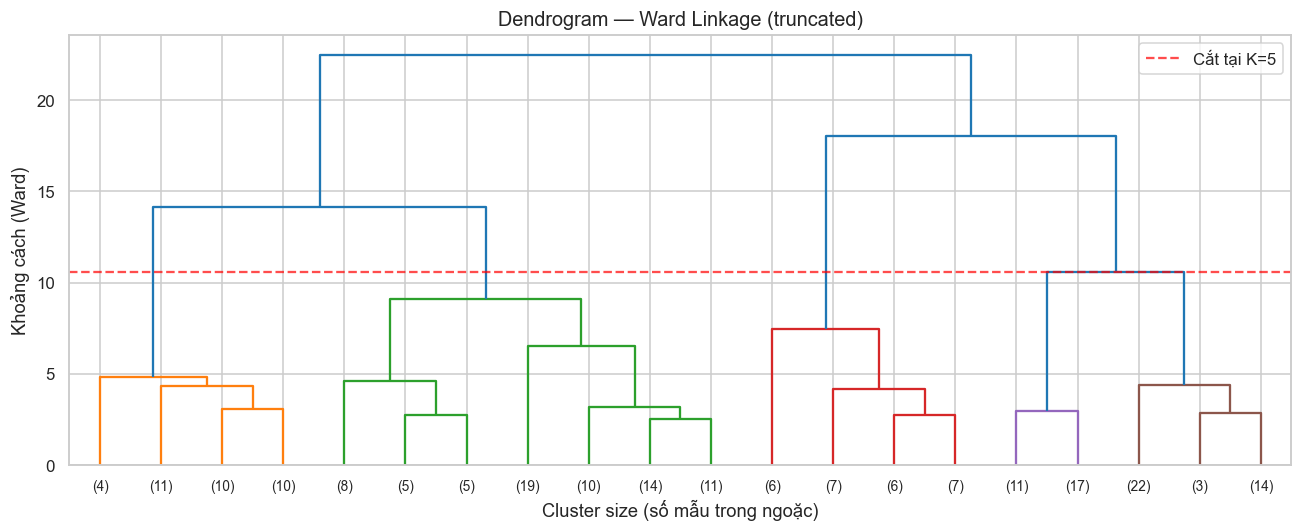
\includegraphics[width=\textwidth]{figures/fig_06.png}
    \caption{Dendrogram (Ward linkage, truncated at 20 leaves). Red dashed line indicates the cut for $K = 5$}
    \label{fig:dendrogram}
\end{figure}

Figure~\ref{fig:hierscatter} shows the hierarchical clustering result using the same axes as Figure~\ref{fig:kmeansscatter}. The cluster boundaries are visually similar to those produced by K-Means.

\begin{figure}[H]
    \centering
    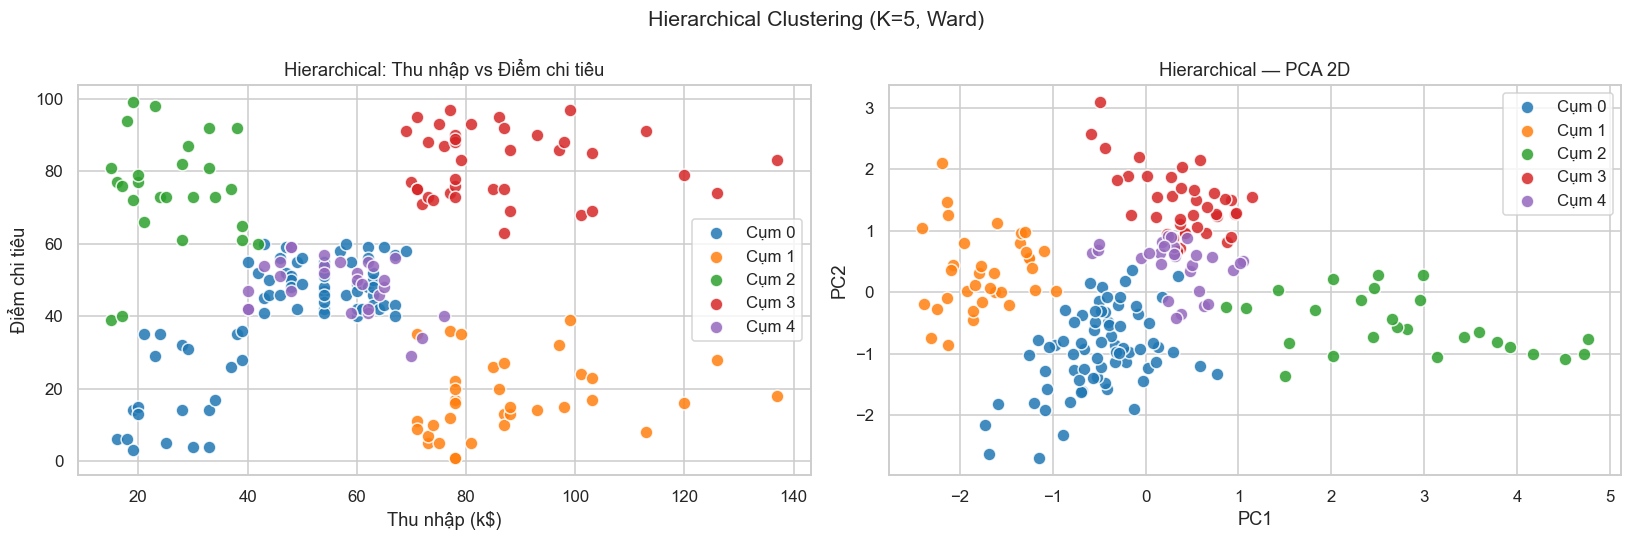
\includegraphics[width=\textwidth]{figures/fig_07.png}
    \caption{Hierarchical clustering result: Income vs.\ Spending Score (left) and PCA 2D projection (right)}
    \label{fig:hierscatter}
\end{figure}

The Hierarchical model performance metrics for $K = 5$ are:
\begin{itemize}
    \item Silhouette Score: \textbf{0.3788}
    \item Davies-Bouldin Index: \textbf{0.8393}
    \item Cluster sizes: 72, 35, 26, 39, 28 customers
\end{itemize}

\subsection{Visualization of Clusters}

\textbf{Principal Component Analysis (PCA)} is applied to reduce the feature space to two dimensions. This allows clusters to be visualized on a two-dimensional scatter plot.

Visualization helps to:

\begin{itemize}
    \item Observe cluster separation.
    \item Detect overlapping groups.
    \item Interpret customer segments more easily.
\end{itemize}

\subsection{Training Output}

After applying the clustering algorithms, each customer in the dataset is assigned a cluster label. These labels represent different customer segments based on demographic and behavioral characteristics.

The clustering results will then be analyzed and compared in the next section to determine which model provides better segmentation performance.

% ----------------------------------------------------

\section{Model Comparison}

\subsection{Evaluation Criteria}

Since clustering is an unsupervised learning task, traditional evaluation metrics such as accuracy or precision cannot be applied. Therefore, internal validation metrics are used to evaluate clustering quality.

Two metrics are used in this project:

\begin{itemize}
    \item \textbf{Silhouette Score}: Measures how well each data point fits within its assigned cluster compared to other clusters. Values range from $-1$ to $1$; higher is better.
    \item \textbf{Davies-Bouldin Index}: Measures the average similarity ratio of each cluster with its most similar cluster. Values $\geq 0$; lower is better.
\end{itemize}

Additionally, the \textbf{Adjusted Rand Index (ARI)} and \textbf{Normalized Mutual Information (NMI)} are used to assess the degree of agreement between the two clustering methods. Although ARI and NMI are typically used when ground truth labels are available, in this project they are used to measure the agreement between the clustering assignments produced by the two algorithms.

\subsection{Clustering Results}

Both clustering algorithms were applied to the standardized dataset using the selected features:

\begin{itemize}
    \item Age, Annual Income, Spending Score, Spending\_Score\_Per\_Income
\end{itemize}

The optimal number of clusters was determined as $K = 5$ using the Elbow Method and dendrogram analysis. The evaluation results are summarized in Table~\ref{tab:comparison}.

\begin{table}[H]
\centering
\begin{tabular}{lcc}
\toprule
\textbf{Model} & \textbf{Silhouette Score} $\uparrow$ & \textbf{Davies-Bouldin Index} $\downarrow$ \\
\midrule
K-Means Clustering ($K=5$)         & \textbf{0.4105} & 0.8508 \\
Hierarchical Clustering ($K=5$)    & 0.3788          & \textbf{0.8393} \\
\bottomrule
\end{tabular}
\caption{Comparison of clustering models at $K = 5$}
\label{tab:comparison}
\end{table}

Figure~\ref{fig:silcomparison} compares the Silhouette Score of both models across all tested values of $K$. K-Means consistently achieves higher or comparable silhouette scores across the range.

\begin{figure}[H]
    \centering
    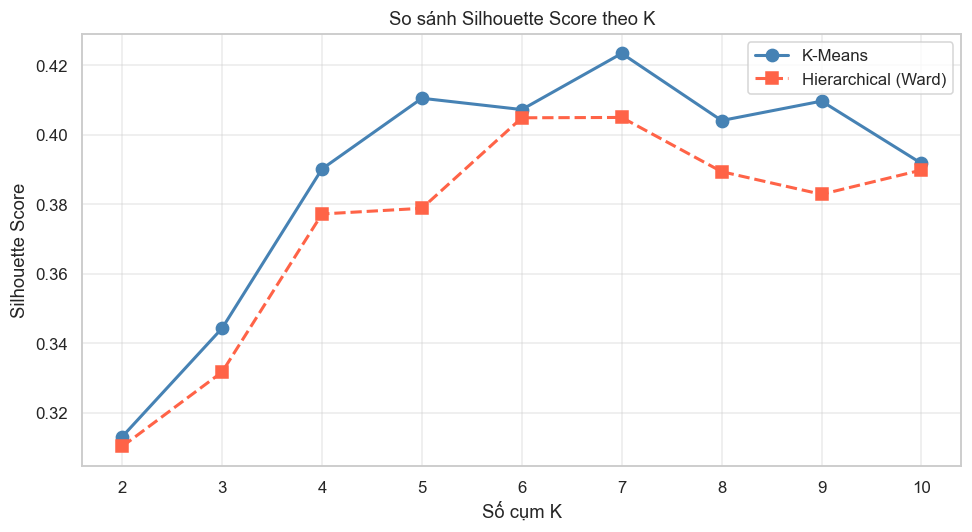
\includegraphics[width=0.75\textwidth]{figures/fig_08.png}
    \caption{Silhouette Score comparison between K-Means and Hierarchical Clustering for $K = 2$ to $10$}
    \label{fig:silcomparison}
\end{figure}

To further validate the consistency between the two methods, the Adjusted Rand Index (ARI) and Normalized Mutual Information (NMI) were computed between the two sets of cluster labels:

\begin{itemize}
    \item Adjusted Rand Index: \textbf{0.7726}
    \item Normalized Mutual Information: \textbf{0.8473}
\end{itemize}

Both values are close to 1.0, indicating that the two methods produce highly consistent segmentation results. This confirms that the five-cluster structure is stable and not an artifact of a particular algorithm.

\subsection{Cluster Profiling}

Figure~\ref{fig:radar} shows radar charts for each of the five clusters, illustrating their normalized profiles across all four features. The charts reveal clearly differentiated segments with distinct behavioral patterns.

\begin{figure}[H]
    \centering
    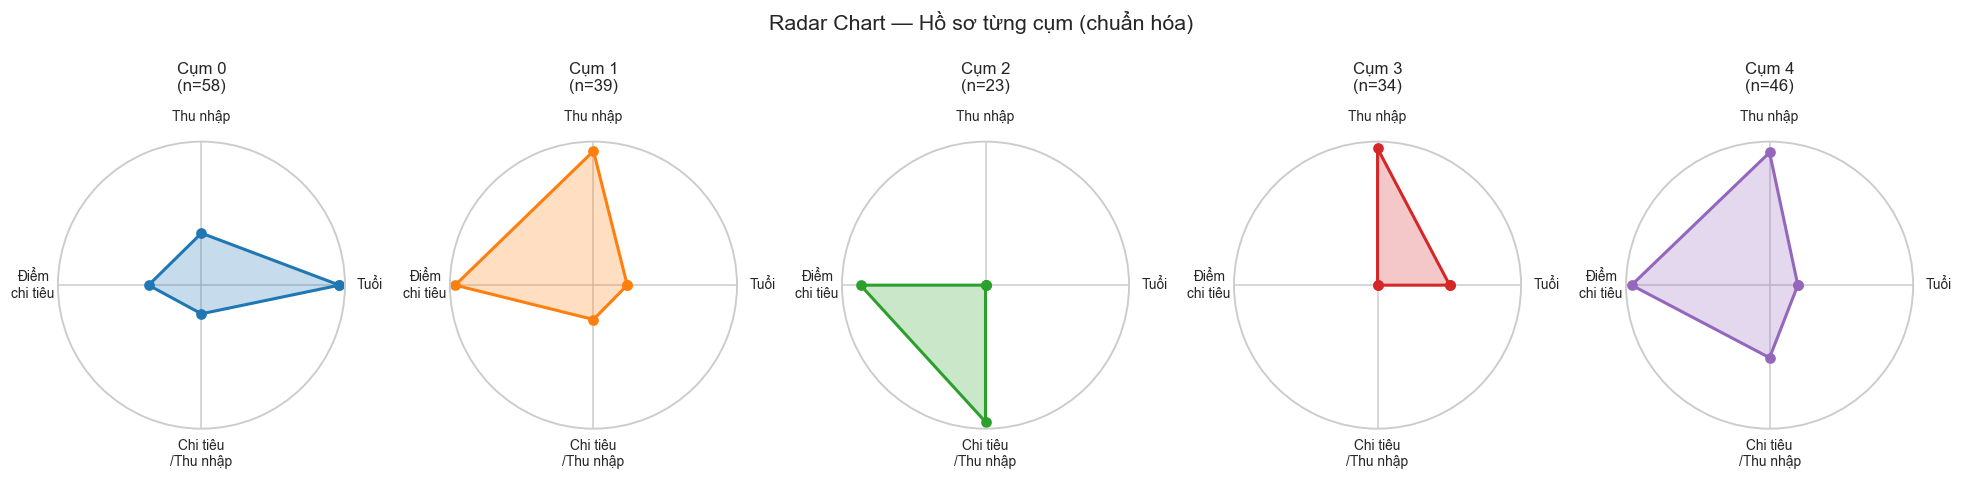
\includegraphics[width=\textwidth]{figures/fig_09.png}
    \caption{Radar charts of normalized cluster profiles (K-Means, $K = 5$)}
    \label{fig:radar}
\end{figure}

Figure~\ref{fig:barchart} compares the mean Annual Income and mean Spending Score of each cluster, providing a clear view of the economic behavior of each segment.

\begin{figure}[H]
    \centering
    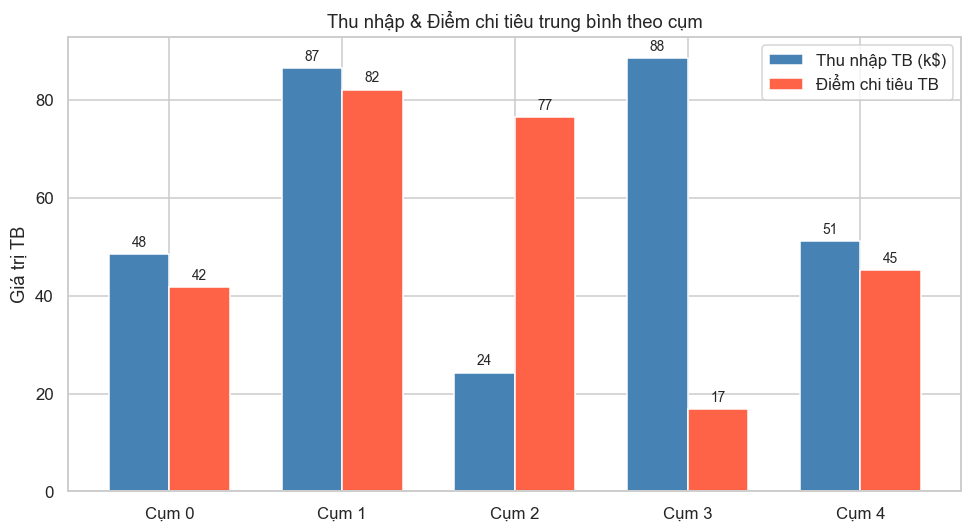
\includegraphics[width=0.75\textwidth]{figures/fig_10.png}
    \caption{Mean Annual Income and Spending Score per cluster}
    \label{fig:barchart}
\end{figure}

\subsection{Interpretation}

Based on the silhouette scores, the K-Means clustering model achieved a higher silhouette score (0.4105) compared to the hierarchical clustering model (0.3788). This suggests that K-Means produced more compact and better-separated clusters under this feature set.

However, the Davies-Bouldin Index for Hierarchical Clustering is marginally lower (0.8393 vs.\ 0.8508), indicating slightly better inter-cluster separability in that metric. The difference is small and both methods are considered competitive.

Additionally, the visualization results using PCA show clear cluster separation in both methods, further validating the five-cluster structure.

The hierarchical clustering dendrogram provides an additional advantage: it reveals the hierarchical relationships between data points and allows analysts to select different granularities of segmentation without retraining.

\subsection{Advantages and Limitations}

Each model has its own strengths and limitations:

\textbf{K-Means Advantages}

\begin{itemize}
    \item Computationally efficient for larger datasets.
    \item Produces well-defined spherical clusters.
    \item Easy to interpret and widely used in business applications.
\end{itemize}

\textbf{K-Means Limitations}

\begin{itemize}
    \item Requires the number of clusters to be predefined.
    \item Sensitive to initialization and outliers.
\end{itemize}

\textbf{Hierarchical Clustering Advantages}

\begin{itemize}
    \item Does not require a predefined number of clusters initially.
    \item Provides a dendrogram that helps visualize cluster relationships.
\end{itemize}

\textbf{Hierarchical Clustering Limitations}

\begin{itemize}
    \item Computationally expensive for large datasets.
    \item Once clusters are merged, they cannot be split again.
\end{itemize}

\subsection{Final Model Selection}

Considering the silhouette score, visualization results, and computational efficiency, the \textbf{K-Means clustering model} is selected as the final model for customer segmentation in this project.

This model provides clearer cluster separation and is more suitable for practical deployment in marketing analysis and customer segmentation tasks.

Figure~\ref{fig:finalsegments} shows the final segmentation result with each cluster labeled by its business interpretation.

\begin{figure}[H]
    \centering
    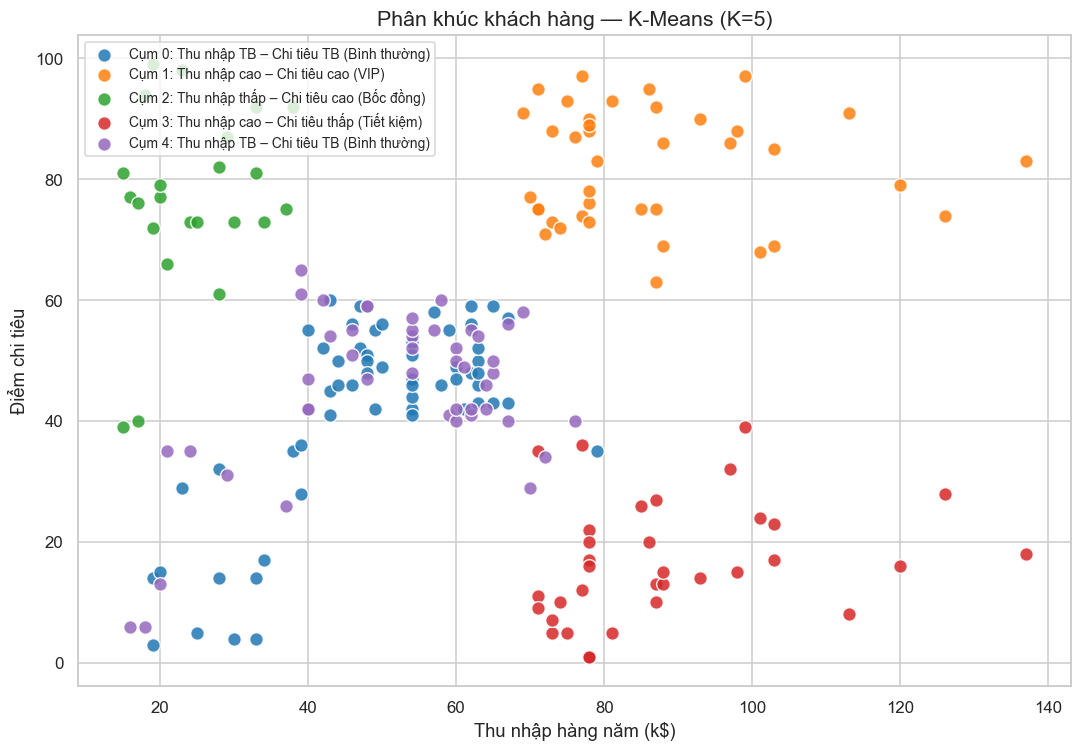
\includegraphics[width=0.75\textwidth]{figures/fig_11.png}
    \caption{Final customer segmentation result (K-Means, $K = 5$) with business segment labels}
    \label{fig:finalsegments}
\end{figure}

\subsection{Business Insight}

Based on the clustering results, five distinct customer segments were identified:

\begin{itemize}
    \item \textbf{High Income -- High Spending (VIP)}: Top-priority customers for premium loyalty programs and exclusive offers.
    \item \textbf{Low Income -- High Spending (Impulsive)}: Highly responsive to flash sales, limited-time offers, and FOMO marketing.
    \item \textbf{High Income -- Low Spending (Conservative)}: Untapped premium segment; can be activated through personalized value propositions.
    \item \textbf{Low Income -- Low Spending (Cautious)}: Price-sensitive group; best targeted through value-for-money promotions.
    \item \textbf{Middle Income -- Middle Spending (Standard)}: Core customer group; suitable for standard upsell and membership programs.
\end{itemize}

By leveraging these insights, the shopping mall can implement more effective and data-driven marketing strategies tailored to each segment's behavior and financial profile.

% ----------------------------------------------------

\section{Conclusion}

\subsection{Summary}

This project applied unsupervised machine learning techniques to perform customer segmentation on the Mall Customers dataset. The objective was to group 200 customers into meaningful segments based on demographic and behavioral features, including Age, Annual Income, and Spending Score, augmented by the derived feature Spending\_Score\_Per\_Income.

Two clustering algorithms were evaluated: K-Means and Hierarchical Clustering (Agglomerative, Ward linkage), both configured at $K = 5$ clusters as determined by the Elbow Method, Silhouette Score analysis, and dendrogram inspection.

The key findings are as follows:

\begin{itemize}
    \item K-Means achieved a higher Silhouette Score (0.4105 vs.\ 0.3788), indicating more compact and internally consistent clusters.
    \item Hierarchical Clustering achieved a marginally lower Davies-Bouldin Index (0.8393 vs.\ 0.8508), reflecting slightly better inter-cluster separability on that metric.
    \item Both methods produced highly consistent segmentation results, as confirmed by an ARI of 0.7726 and NMI of 0.8473.
    \item Five distinct customer segments were identified: VIP, Impulsive, Conservative, Cautious, and Standard customers.
\end{itemize}

\subsection{Model Selection}

K-Means is selected as the final model due to its higher Silhouette Score, well-separated cluster visualization in PCA space, and greater computational efficiency. The feature engineering step, in particular the introduction of Spending\_Score\_Per\_Income, contributed to more nuanced segmentation by capturing the relationship between earning capacity and purchasing behavior.

\subsection{Business Implications}

The five identified segments provide actionable insights for the mall management:

\begin{itemize}
    \item The VIP segment should be prioritized for exclusive loyalty programs and premium offerings.
    \item The Impulsive segment responds well to time-limited promotions and urgency-based marketing.
    \item The Conservative segment represents an untapped premium opportunity that can be activated through personalized value propositions.
    \item The Cautious segment requires value-driven communication and cost-effective promotions.
    \item The Standard segment, being the largest core group, is well-suited for standard membership programs and general upselling.
\end{itemize}

By deploying data-driven segmentation, the organization can move away from one-size-fits-all marketing and instead allocate its budget more precisely across segments that differ in financial capacity and behavioral propensity.

\subsection{Limitations and Future Work}

Several limitations are acknowledged:

\begin{itemize}
    \item The dataset is relatively small (200 records), which may limit the generalizability of the results to larger and more diverse customer populations.
    \item K-Means assumes spherical cluster shapes, which may not always reflect real-world customer distributions.
    \item The current feature set does not include transactional data (e.g., purchase frequency, average basket size), which could further improve segmentation quality.
\end{itemize}

Future work could explore density-based methods such as DBSCAN to handle non-spherical clusters, incorporate richer behavioral features from transaction histories, and apply semi-supervised or temporal clustering to track how customer segments evolve over time.

\end{document}
